\documentclass[
]{jss}

\usepackage[utf8]{inputenc}

\providecommand{\tightlist}{%
  \setlength{\itemsep}{0pt}\setlength{\parskip}{0pt}}

\author{
Sahir Rai Bhatnagar*\\McGill University \And Maxime Turgeon*\\University of Manitoba \AND Jesse Islam\\McGill University \And James Hanley\\McGill University \And Olli Saarela\\University of Toronto
}
\title{\pkg{casebase}: An Alternative Framework For Survival Analysis}

\Plainauthor{Sahir Rai Bhatnagar*, Maxime Turgeon*, Jesse Islam, James Hanley, Olli Saarela}
\Plaintitle{casebase: An Alternative Framework For Survival Analysis}
\Shorttitle{\pkg{casebase}: An Alternative Framework For Survival Analysis}

\Abstract{
The abstract of the article. *SRB and MT contributed equally to this
work.
}

\Keywords{survival analysis, absolute risk, data visualization}
\Plainkeywords{survival analysis, absolute risk, data visualization}

%% publication information
%% \Volume{50}
%% \Issue{9}
%% \Month{June}
%% \Year{2012}
%% \Submitdate{}
%% \Acceptdate{2012-06-04}

\Address{
    Sahir Rai Bhatnagar*\\
  McGill University\\
  1020 Pine Avenue West Montreal, QC, Canada H3A 1A2\\
  E-mail: \email{sahir.bhatnagar@mail.mcgill.ca}\\
  URL: \url{http://sahirbhatnagar.com/}\\~\\
      Maxime Turgeon*\\
  University of Manitoba\\
  186 Dysart Road Winnipeg, MB, Canada R3T 2N2\\
  E-mail: \email{max.turgeon@umanitoba.ca}\\
  URL: \url{https://maxturgeon.ca/}\\~\\
      Jesse Islam\\
  McGill University\\
  1020 Pine Avenue West Montreal, QC, Canada H3A 1A2\\
  E-mail: \email{jesse.islam@mail.mcgill.ca}\\
  
      James Hanley\\
  McGill University\\
  1020 Pine Avenue West Montreal, QC, Canada H3A 1A2\\
  E-mail: \email{james.hanley@mcgill.ca}\\
  URL: \url{http://www.medicine.mcgill.ca/epidemiology/hanley/}\\~\\
      Olli Saarela\\
  University of Toronto\\
  Dalla Lana School of Public Health, 155 College Street, 6th floor,
  Toronto, Ontario M5T 3M7, Canada\\
  E-mail: \email{olli.saarela@utoronto.ca}\\
  URL: \url{http://individual.utoronto.ca/osaarela/}\\~\\
  }


% Pandoc header

\usepackage{amsmath} \usepackage{longtable} \usepackage{graphicx} \usepackage{tabularx} \usepackage{float} \usepackage{booktabs} \usepackage{makecell} \usepackage{tabu} \DeclareUnicodeCharacter{2500}{-}

\begin{document}

\hypertarget{introduction}{%
\section{Introduction}\label{introduction}}

Survival analysis has been greatly influenced over the last 50 years by
the partial likelihood approach of the Cox proportional hazard model
\citep{cox1972regression}. This approach provides a flexible way of
assessing the influence of covariates on the hazard function, without
the need to specify a parametric survival model. This flexibility comes
at the cost of decoupling the baseline hazard from the effect of the
covariates. To recover the whole survival curve---or the cumulative
incidence function (CIF)---we then need to separately estimate the
baseline hazard \citep{breslow1972discussion}. This in turn often leads
to stepwise estimates of the survival function.

From the perspective of clinicians and their patients, the most relevant
quantity is often the 5- or 10-year risk of having a certain event given
the patient's particular circumstances, and not the hazard ratio between
a treatment and control group. Therefore, to make sound clinical
decisions, it is important to accurately estimate the \emph{full} hazard
function, which can then be used to estimate the cumulative incidence
function (CIF). Since the parametric hazard is a smooth function of
time, the CIF and the survival function estimates also vary smoothly
over time.

With the goal of fitting smooth-in-time hazard functions, Hanley \&
Miettinen \citeyearpar{hanley2009fitting} proposed a general framework
for estimating fully parametric hazard models via logistic regression.
Their approach provides users that are familiar with generalized linear
models with a natural way of fitting parametric survival models.
Moreover, their framework is very flexible: general functions of time
can be estimated (e.g.~using splines or general additive models), and
hence these models retain some of the flexibility of partial likelihood
approaches.

In this article, we present an \proglang{R} package that combines the
ideas of Hanley \& Miettinen into a simple interface. The purpose of the
\pkg{casebase} package is to provide practitioners with an easy-to-use
software tool to predict the risk (or cumulative incidence) of an event,
conditional on a particular patient's covariate profile. Our package
retains the flexibility of case-base sampling and the familiar interface
of the \code{glm} function. In addition, we provide extensive
visualization tools.

In what follows, we first recall some theoretical details on case-base
sampling and its use for estimating parametric hazard functions. We then
give a short review of existing \proglang{R} packages that implement
comparable features as \pkg{casebase}. Next, we provide some details
about the implementation of case-base sampling in our package, and we
give a brief survey of its main functions. This is followed by four case
studies that illustrate the flexibility and capabilities of
\pkg{casebase}. We show how the same framework can be used for competing
risk analyses, penalized estimation, and for studies with time-dependent
exposures. Finally, we end the article with a discussion of the results
and of future directions.

\hypertarget{theory}{%
\section{Theoretical details}\label{theory}}

As discussed in Hanley \& Miettinen \citeyearpar{hanley2009fitting}, the
key idea behind case-base sampling is to discretize the study base into
an infinite amount of \emph{person moments}. These person moments are
indexed by both an individual in the study and a time point, and
therefore each person moment has a covariate profile, an exposure status
and an outcome status attached to it. We note that there is only a
finite number of person moments associated with the event of interest
(what Hanley \& Miettinen call the \emph{case series}). Case-base
sampling refers to the sampling from the base of a representative finite
sample called the \emph{base series}.

To describe the theoretical foundations of case-base sampling, we use
the framework of counting processes. In what follows, we abuse notation
slightly and omit any mention of \(\sigma\)-algebras; the interested
reader can refer to Saarela \& Arjas \citeyearpar{saarela2015non} and
Saarela \citeyearpar{saarela2016case}. First, let
\(N_{i}(t) \in \{0, 1\}\) be counting processes corresponding to the
event of interest for individual \(i=1, \ldots,n\). For simplicity, we
will consider Type I censoring due to the end of follow-up at time
\(\tau\) (the general case of non-informative censoring is treated in
Saarela \citeyearpar{saarela2016case}). We assume a continuous time
model, which implies that the counting process jumps are less than or
equal to one. We are interested in modeling the hazard functions
\(\lambda_{i}(t)\) of the processes \(N_i(t)\), and which satisfy
\[\lambda_{i}(t) dt = E[dN_{i}(t)].\]

Next, we model the base series sampling mechanism using non-homogeneous
Poisson processes \(R_i(t) \in \{0, 1, 2, \ldots\}\), with the
person-moments where \(dR_i(t) = 1\) constituting the base series. The
process \(Q_{i}(t) = R_i(t) + N_{i}(t)\) then counts both the case and
base series person-moments contributed by individual \(i\). This process
is typically defined by the user via its hazard function \(\rho_i(t)\).
The process \(Q_{i}(t)\) is characterized by
\(E[dQ_{i}(t)] = \lambda_{i}(t)dt + \rho_i(t)dt\).

If the hazard function \(\lambda_{i}(t; \theta)\) is parametrized in
terms of \(\theta\), we could define an estimator \(\hat{\theta}\) by
maximization of the likelihood expression
\[L_0(\theta) = \prod_{i=1}^n \exp\left\{ -\int_0^\tau \lambda_i(t; \theta) dt \right\} \prod_{i=1}^{n} \prod_{t\in[0,\tau)} \lambda_{i}(t;\theta)^{dN_{i}(t)}\left(1 - \lambda_{i}(t;\theta)\right)^{1 - dN_{i}(t)},\]
where \(\prod_{t\in[0,u)}\) represents a product integral from \(0\) to
\(u\). However, the integral over time makes the computation and
maximization of \(L_0(\theta)\) challenging.

Case-base sampling allows us to avoid this integral. By conditioning on
a sampled person-moment, we get individual contributions of the form
\[P(dN_{i}(t) \mid dQ_{i}(t) = 1) \stackrel{\theta}{\propto} \frac{\lambda_{i}(t; \theta)^{dN_{i}(t)}}{\rho_i(t) + \lambda_{i}(t;\theta)}.\]
Therefore, we can define an estimating equation for \(\theta\) as
follows:
\[L(\theta) = \prod_{i=1}^{n} \prod_{t\in[0,\tau)} \left(\frac{\lambda_{i}(t; \theta)^{dN_{i}(t)}}{\rho_i(t) + \lambda_{i}(t;\theta)}\right)^{dQ_i(t)}.\]
When a logarithmic link function is used for modeling the hazard
function, the above expression is of a logistic regression form with an
offset term \(\log(1/\rho_i(t))\). Note that the sampling units selected
in the case-base sampling mechanism are person-moments, rather than
individuals, and the parameters to be estimated are hazards or hazard
ratios rather than odds or odds ratios. Generally, an individual can
contribute more than one person-moment, and thus the terms in the
product integral are not independent. Nonetheless, Saarela
\citeyearpar{saarela2016case} showed that the logarithm of this
estimating function has mean zero at the true value \(\theta=\theta_0\),
and that the resulting estimator \(\hat{\theta}\) is asymptotically
normally distributed.

In Hanley \& Miettinen \citeyearpar{hanley2009fitting}, the authors
suggest sampling the base series \emph{uniformly} from the study base.
In terms of Poisson processes, their sampling strategy corresponds
essentially to a time-homogeneous Poisson process with hazard equal to
\(\rho_i(t) = b/B\), where \(b\) is the number of sampled observations
in the base series, and \(B\) is the total population-time for the study
base (e.g.~the sum of all individual follow-up times). More complex
examples are also possible; see for example Saarela \& Arjas
\citeyearpar{saarela2015non}, where the intensity functions for the
sampling mechanism are proportional to the cardiovascular disease event
rate given by the Framingham score. With this sampling mechanism,
Saarela \& Arjas are able to increase the efficiency of their
estimators, when compared to uniform sampling.

Let \(g(t; X)\) be the linear predictor such that
\(\log(\lambda(t;X)) = g(t; X)\). Different functions of \(t\) lead to
different parametric hazard models. The simplest of these models is the
one-parameter exponential distribution which is obtained by taking the
hazard function to be constant over the range of \(t\):

\begin{equation}
\log(\lambda(t; X)) = \beta_0 + \beta_1 X. \label{eq:exp}
\end{equation}

In this model, the instantaneous failure rate is independent of
\(t\).\footnote{The conditional chance of failure in a time interval of specified length is the same regardless of how long the individual has been in the study. This is also known as the \textit{memoryless property} \citep{kalbfleisch2011statistical}.}

The Gompertz hazard model is given by including a linear term for time:

\begin{equation}
\log(\lambda(t; X)) = \beta_0 + \beta_1 t + \beta_2 X. \label{eq:gomp}
\end{equation}

Use of \(\log(t)\) yields the Weibull hazard which allows for a power
dependence of the hazard on time \citep{kalbfleisch2011statistical}:

\begin{equation}
\log(\lambda(t; X)) = \beta_0 + \beta_1 \log(t) + \beta_2 X. \label{eq:weibull}
\end{equation}

Case-base sampling can also be used in the context of competing-risk
analyses. Assuming there are \(J\) competing events, we can show that
each person-moment's contribution of the likelihood is of the form

\[\frac{\lambda_j(t)^{dN_j(t)}}{\rho(t) + \sum_{j=1}^J\lambda_j(t)},\]

where \(N_j(t)\) is the counting process associated with the event of
type \(j\) and \(\lambda_j(t)\) is the corresponding hazard function. As
may be expected, this functional form is similar to the terms appearing
in the likelihood function for multinomial
regression.\footnote{Specifically, it corresponds to the following parametrization: \begin{align*} \log\left(\frac{P(Y=j \mid X)}{P(Y = J \mid X)}\right) = X^T\beta_j, \qquad j = 1,\ldots, J-1.\end{align*}}

\hypertarget{existing-packages}{%
\section{Existing packages}\label{existing-packages}}

Survival analysis is an important branch of applied statistics and
epidemiology. Accordingly, there is already a vast ecosystem of \code{R}
packages implementing different methodologies. In this section, we
describe how the functionalities of \pkg{casebase} compare to these
packages.

At the time of writing, a cursory examination of CRAN's task view on
survival analysis reveals that there are over 250 packages related to
survival analysis \citeyearpar{survTaskView}. For the purposes of this
article, we restricted our review to packages that implement at least
one of the following features: parametric modeling, non-proportional
hazard models, competing risk analysis, penalized estimation, and CIF
estimation. By searching for appropriate keywords in the
\code{DESCRIPTION} file of these packages, we found 60 relevant
packages. These 60 packages were then manually examined to determine
which ones are comparable to \pkg{casebase}. In particular, we excluded
packages that were focused on a different set of problems, such as
frailty and multi-state models. The remaining 14 packages appear in
Table \ref{tab:surv-pkgs}, along with some of the functionalities they
offer.

Parametric survival models are implemented in a handful of packages:
\pkg{CFC} \citeyearpar{mahani2015bayesian}, \pkg{flexsurv}
\citeyearpar{flexsurv}, \pkg{SmoothHazard} \citeyearpar{smoothHazard},
\pkg{rsptm2} \citeyearpar{clements_liu}, \pkg{mets}
\citeyearpar{scheike2014estimating}, and \pkg{survival}
\citeyearpar{survival-package}. The types of models they allow vary for
each package. For example, \pkg{SmoothHazard} is limited to Weibull
distributions \citeyearpar{smoothHazard}, whereas both \pkg{flexsurv}
and \pkg{survival} allow users to supply any distribution of their
choice. Also, \pkg{flexsurv}, \pkg{smoothhazard}, \pkg{mets} and
\pkg{rstpm2} also have the ability to model the effect of time using
splines, which allows flexible modeling of the hazard function.
Moreover, \pkg{flexsurv} has the ability to estimate both scale and
shape parameters for a variety of parametric families. As discussed
above, \pkg{casebase} can model any parametric family whose log-hazard
can be expressed as a linear combination of covariates (including time).
Therefore, our package allows the user to model the effect of time using
splines. Also, by including interaction terms between covariates and
time, it also allows users to fit time-varying coefficient models.
However, we do not explicitly model any shape parameter, unlike
\pkg{flexsurv}.

Several packages implement penalized estimation for the Cox model:
\pkg{glmnet} \citeyearpar{regpathcox}, \pkg{glmpath}
\citeyearpar{park_hastie}, \pkg{penalized} \citeyearpar{l1penal},
\pkg{riskRegression} \citeyearpar{gerds_blanche}. Moreover, some
packages also include penalized estimation in the context of Cox models
with time-varying coefficients: elastic-net penalization with
\pkg{CoxRidge} \citeyearpar{perperoglou} and \pkg{rstpm2}
\citeyearpar{clements_liu}, while \pkg{survival}
\citeyearpar{survival-package} has an implementation of ridge-penalized
estimation. On the other hand, our package \pkg{casebase} provides
penalized estimation in the context of parametric hazards. To our
knowledge, \pkg{casebase} and \pkg{rsptm2} are the only packages to
offer this functionality.

Next, several \proglang{R} packages implement methodologies for
competing risk analysis; for a different perspective on this topic, see
Mahani \& Sharabiani \citeyearpar{mahani2015bayesian}. The package
\pkg{cmprsk} provides methods for cause-specific subdistributions, such
as in the Fine-Gray model \citeyearpar{fine1999proportional}. On the
other hand, the package \pkg{CFC} estimates cause-specific CIFs from
unadjusted, non-parametric survival functions. Our package
\pkg{casebase} also provides functionalities for competing risk analysis
by estimating parametrically the cause-specific hazards. From these
quantities, we can then estimate the cause-specific CIFs.

Finally, several packages include functions to estimate the CIF. The
corresponding methods generally fall into two categories: transformation
of the estimated hazard function, and semi-parametric estimation of the
baseline hazard. The first category broadly corresponds to parametric
survival models, where the full hazard is explicitly modeled. Using this
estimate, the survival function and the CIF can be obtained using their
functional relationships (see Equations \ref{eqn:surv} and \ref{eqn:CI}
below). Packages providing this functionality include \pkg{CFC},
\pkg{flexsurv}, \pkg{mets}, and \pkg{survival}. Our package
\pkg{casebase} also follows this approach for both single-event and
competing-risk analyses. The second category outlined above broadly
corresponds to semi-parametric models. These models do not model the
full hazard function, and therefore the baseline hazard needs to be
estimated separately in order to estimate the survival function. This is
achieved using semi-parametric estimators (e.g.~Breslow's estimator) or
parametric estimators (e.g.~spline functions). Packages that implement
this approach include \pkg{RiskRegression}, \pkg{rstpm2}, and
\pkg{survival}. As mentioned in the introduction, a key distinguishing
factor between these two approaches is that the first category leads to
smooth estimates of the cumulative incidence function, whereas the
second category often produces estimates in the form of step-wise
functions. Providing smooth estimates of the CIF was one of the main
motivations for introducing case-base sampling in survival analysis.

\begin{table}[ht]
\centering
\resizebox{\textwidth}{!}{%
\begin{tabular}{ccccccccc}
\hline
& \textbf{Competing} & \textbf{Allows} &  \textbf{Penalized}   &    &  & \textbf{Semi} & \textbf{Interval/Left} & \textbf{Absolute}  \\
\textbf{Package}        & \textbf{Risks}  & \textbf{Non PH} & \textbf{Regression} & \textbf{Splines} & \textbf{Parametric} & \textbf{Parametric} & \textbf{Censoring} & \textbf{Risk}           \\
\hline
\textbf{casebase}        & x                        & x                         & x                     & x                & x                   &                          &                                  & x                                \\ \bottomrule
\textbf{CFC}             & x                        & x                         &                       &                  & x                   &                          &                                  & x                                \\ \bottomrule
\textbf{cmprsk}             & x                        &                           &                       &                  &                     &  x                        &                                  & x                                \\ \bottomrule
\textbf{CoxRidge}        &                          & x                         & x                     &                  &                     & x                        &                                  &                                  \\ \bottomrule
\textbf{crrp}            & x                        &                           & x                     &                  &                     & x                        &                                  &                                  \\ \bottomrule
\textbf{fastcox}         &                          &                           & x                     &                  &                     & x                        &                                  &                                  \\ \bottomrule
\textbf{flexrsurv}       &                          & x                         &                       & x                & x                   &                          &                                  & x               \\ \bottomrule
\textbf{flexsurv}        & x                        & x                         &                       & x                & x                   &                          &                                  & x               \\ \bottomrule
\textbf{glmnet}          &                          &                           & x                     &                  &                     & x                        &                                  &                                  \\ \bottomrule
\textbf{glmpath}         &                          &                           & x                     &                  &                     & x                        &                                  &                                  \\ \bottomrule
\textbf{mets}            & x                        &                           &                       & x                &                     & x                        &                                  & x                                \\ \bottomrule
\textbf{penalized}       &                          &                           & x                     &                  &                     & x                        &                                  &                                  \\ \bottomrule
\textbf{riskRegression}  & x                         &                           & x                     &                  &                     & x                        &                                  & x                                \\ \bottomrule
\textbf{rstpm2}          &                          & x                         &                      & x                & x                   & x                        & x                                & x                         \\ \bottomrule
\textbf{SmoothHazard}    &                          & x                         &                       & x                & x                   &                          & x                            &                                      \\ \bottomrule
\textbf{survival}        & x                        & x                         &                       &                  & x                   & x                        & x                                & x                               \\ \bottomrule
\hline
\end{tabular}%
}
\caption{Comparison of various \proglang{R} packages for survival analysis based on several defining features. Competing Risks: whether or not an implementation for competing risks is present. Allows Non-PH: permits models that can incorporate variables that change with survival time. Penalized Regression: allows for a penalty term when fitting the model. This is not restricted to lasso nor ridge. Splines: the package permits a flexible fit on time through the use of splines. Parametric: the package has implementations for parametric models. Semi-parametric: the package has implementations for semi-parametric models. Interval/left censoring: the package can interpret interval and left-censoring. If this is not selected, the package only handles right-censoring. Absolute Risk: the package has an implementation for survival curves, cumulative incidence or cumulative hazard rate functions to be plotted.}
\label{tab:surv-pkgs}
\end{table}

\hypertarget{implementation-details}{%
\section{Implementation details}\label{implementation-details}}

The functions in the \pkg{casebase} package can be divided into two
categories: 1) exploratory data analysis, in the form of population-time
plots; and 2) parametric modeling of the hazard function. We strove for
compatibility with both \code{data.frame}s and \code{data.table}s; this
can be seen in the coding choices we made and the unit tests we wrote.

\hypertarget{population-time-plots}{%
\subsection{Population-time plots}\label{population-time-plots}}

The case-base sampling approach described in Section \ref{theory} can be
visualized in the form of a population time plot. These plots are
extremely informative graphical displays of survival data and should be
one of the first steps in an exploratory data analysis. The
\code{popTime} function and \code{plot} method facilitate this task:

\begin{enumerate}
\def\labelenumi{\arabic{enumi}.}
\tightlist
\item
  The \code{casebase::popTime} function takes as input the original
  dataset along with the column names corresponding to the timescale,
  the event status and an exposure group of interest (optional). This
  will create an object of class \code{popTime}.\\
\item
  The corresponding \code{plot} method for the object created in Step 1
  can be called to create the population time plot with several options
  for customizing the aesthetics.
\end{enumerate}

By splitting these tasks, we give flexibility to the user. While the
method call in Step 2 allows further customization by using the
\pkg{ggplot2} \citep{ggplot2} family of functions, users can use for the
graphics system of their choice to create population-time plots from the
object created in Step 1.

To illustrate these functions, we will use the European Randomized Study
of Prostate Cancer Screening (ERSPC) data \citep{schroder2009screening}
which was extracted using the approach described in Liu \emph{et al.}
\citeyearpar{liu2014recovering} This dataset is available through the
\pkg{casebase} package. It contains the individual observations for
159,893 men from seven European countries, who were between the ages of
55 and 69 years when recruited for the trial.

We first create the necessary dataset for producing the population time
plot using the \code{popTime} function. In this example, we stratify the
plot by treatment group. The resulting object inherits from class
\code{popTime} and stores the exposure variable as an attribute:

\begin{CodeChunk}

\begin{CodeInput}
R> pt_object <- casebase::popTime(ERSPC, 
R+                                time = "Follow.Up.Time",
R+                                event = "DeadOfPrCa",
R+                                exposure = "ScrArm")
R> inherits(pt_object, "popTime")
\end{CodeInput}

\begin{CodeOutput}
#> [1] TRUE
\end{CodeOutput}

\begin{CodeInput}
R> attr(pt_object, "exposure")
\end{CodeInput}

\begin{CodeOutput}
#> [1] "ScrArm"
\end{CodeOutput}
\end{CodeChunk}

We then pass this object to the corresponding \code{plot} method:

\begin{CodeChunk}

\begin{CodeInput}
R> plot(pt_object, add.base.series = TRUE)
\end{CodeInput}
\end{CodeChunk}

\begin{CodeChunk}
\begin{figure}

{\centering 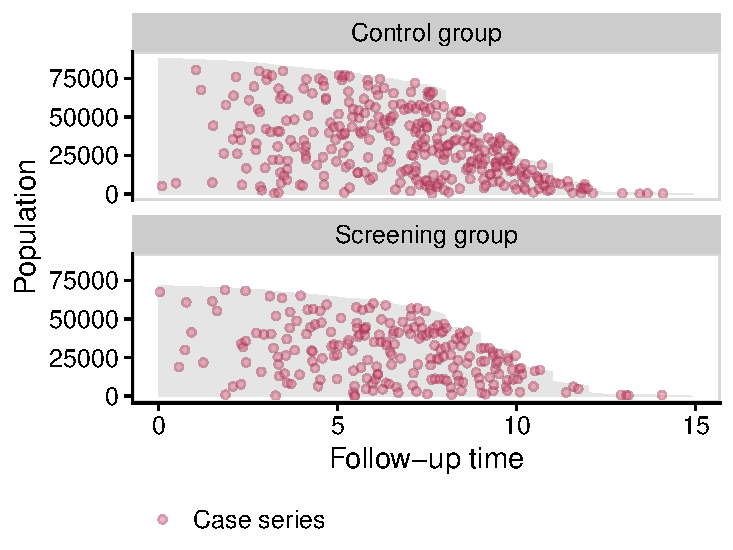
\includegraphics[width=\textwidth,keepaspectratio=true]{../figures/plot-stratified-erspc-data-1} 

}

\caption[Population time plot for ERSPC data]{Population time plot for ERSPC data.}\label{fig:plot-stratified-erspc-data}
\end{figure}
\end{CodeChunk}

Figure \ref{fig:plot-stratified-erspc-data} is built sequentially by
first adding a layer for the area representing the population time in
gray, with subjects having the least amount of observation time plotted
at the top of the y-axis. We immediately notice a distinctive
\emph{step-wise shape} in the population time area. This is due to the
randomization of the Finnish cohorts which were carried out on January 1
of each of year from 1996 to 1999. Coupled with the uniform December 31
2006 censoring date, this led to large numbers of men with exactly 11,
10, 9 or 8 years of follow-up. Tracked backwards in time (i.e.~from
right to left), the population-time plot shows the recruitment pattern
from its beginning in 1991, and the January 1 entries in successive
years. Tracked forwards in time (i.e.~from left to right), the plot for
the first three years shows attrition due entirely to death (mainly from
other causes). Since the Swedish and Belgian centres were the last to
complete recruitment--in December 2003--the minimum potential follow-up
is three years. Tracked further forwards in time (i.e.~after year 3) the
attrition is a combination of deaths and staggered entries. As we can
see, population-time plots summarise a wealth of information about the
study into a simple graph.

Next, layers for the case series and base series are added. The case
series is sampled at random vertically on the plot to avoid having all
points along the upper edge of the gray area. By randomly distributing
the cases, we can get a better sense of the incidence density. In Figure
\ref{fig:plot-stratified-erspc-data}, we see that more events are
observed at later follow-up times. Therefore, a constant hazard model
would not be appropriate in this instance as it would overestimate the
cumulative incidence earlier on in time, and underestimate it later on.
Finally, the base series is sampled horizontally with sampling weight
proportional to their follow-up time. The reader should refer to the
package vignettes for more examples and a detailed description of how to
modify the aesthetics of a population-time plot.

\hypertarget{parametric-modeling}{%
\subsection{Parametric modeling}\label{parametric-modeling}}

The parametric modeling step was separated into three parts:

\begin{enumerate}
\def\labelenumi{\arabic{enumi}.}
\tightlist
\item
  case-base sampling;
\item
  estimation of the smooth hazard function;
\item
  estimation of the CIF.
\end{enumerate}

By separating the sampling and estimation functions, we allow the
possibility of users implementing more complex sampling scheme (as
described in Saarela \citeyearpar{saarela2016case}), or more complex
study designs (e.g.~time-varying exposure).

The sampling scheme selected for \code{sampleCaseBase} was described in
Hanley \& Miettinen \citeyearpar{hanley2009fitting}: we first sample
along the ``person'' axis, proportional to each individual's total
follow-up time, and then we sample a moment uniformly over their
follow-up time. This sampling scheme is equivalent to the following
picture: imagine representing the total follow-up time of all
individuals in the study along a single dimension, where the follow-up
time of the next individual would start exactly when the follow-up time
of the previous individual ends. Then the base series could be sampled
uniformly from this one-dimensional representation of the overall
follow-up time. In any case, the output is a dataset of the same class
as the input, where each row corresponds to a person-moment. The
covariate profile for each such person-moment is retained, and an offset
term is added to the dataset. This output could then be used to fit a
smooth hazard function, or for visualization of the base series.

Next, the fitting function \code{fitSmoothHazard} starts by looking at
the class of the dataset: if it was generated from
\code{sampleCaseBase}, it automatically inherited the class
\code{cbData}. If the dataset supplied to \code{fitSmoothHazard} does
not inherit from \code{cbData}, then the fitting function starts by
calling \code{sampleCaseBase} to generate the base series. In other
words, users can bypass \code{sampleCaseBase} altogether and only worry
about the fitting function \code{fitSmoothHazard}.

The fitting function retains the familiar formula interface of
\code{glm}. The left-hand side of the formula should be the name of the
column corresponding to the event type. The right-hand side can be any
combination of the covariates, along with an explicit functional form
for the time variable. Note that non-proportional hazard models can be
achieved at this stage by adding an interaction term involving time
(cf.~Case Study 4 below). The offset term does not need to be specified
by the user, as it is automatically added to the formula before calling
\code{glm}.

To fit the hazard function, we provide several approaches that are
available via the \code{family} parameter. These approaches are:

\begin{itemize}
\tightlist
\item
  \code{glm}: This is the familiar logistic regression.
\item
  \code{glmnet}: This option allows for variable selection using Lasso
  or elastic-net (cf.~Case Study 3). This functionality is provided
  through the \pkg{glmnet} package \citep{friedman2010jss}.
\item
  \code{gam}: This option provides support for \emph{Generalized
  Additive Models} via the \pkg{mgcv} package
  \citep{hastie1987generalized}.
\item
  \code{gbm}: This option provides support for \emph{Gradient Boosted
  Trees} via the \pkg{gbm} package. This feature is still experimental.
\end{itemize}

In the case of multiple events, the hazard is fitted via multinomial
regression as performed by the \pkg{VGAM} package. We selected this
package for its ability to fit multinomial regression models with an
offset.

Once a model-fit object has been returned by \code{fitSmoothHazard}, all
the familiar summary and diagnostic functions are available:
\code{print}, \code{summary}, \code{predict}, \code{plot}, etc. Our
package provides one more functionality: it computes risk functions from
the model fit. For the case of a single event, it uses the familiar
identity \begin{equation}\label{eqn:surv}
S(t) = \exp\left(-\int_0^t \lambda(u;X) du\right).
\end{equation} The integral is computed using either the
\code{stats::integrate} function or Monte-Carlo integration. The risk
function (or cumulative incidence function) is then defined as
\begin{equation}\label{eqn:CI}
CI(t) = 1 - S(t).
\end{equation}

For the case of a competing-event analysis, the event-specific risk is
computed using the following procedure: first, we compute the overall
survival function (i.e.~for all event types):

\[ S(t) = \exp\left(-\int_0^t \Lambda(u;X) du\right),\qquad \Lambda(t;X) = \sum_{j=1}^J \lambda_j(t;X).\]
From this, we can derive the event-specific subdensities:

\[ f_j(t) = \lambda_j(t)S(t).\]

Finally, by integrating these subdensities, we obtain the event-specific
cumulative incidence functions:

\[ CI_j(t) = \int_0^t f_j(u)du.\] The integrals are computed using
either numerical integration (via the trapezoidal rule) or Monte Carlo
integration. This option is controlled by the argument \code{method} of
the \code{absoluteRisk} function.

In the following sections, we illustrate these functionalities in the
context of four case studies.

\hypertarget{case-study-1european-randomized-study-of-prostate-cancer-screening}{%
\section{Case study 1---European Randomized Study of Prostate Cancer
Screening}\label{case-study-1european-randomized-study-of-prostate-cancer-screening}}

For our first case study, we return to the ERSPC study and investigate
the differences in survival between the control and screening arms. We
fit four models that differ in which functional form of time is used: 1)
excluded from the linear predictor, 2) linear function, 3) log function,
and 4) a smooth function using cubic B-splines. The models are fit using
\code{fitSmoothHazard}. Since the output object from
\code{fitSmoothHazard} inherits from the \code{glm} class, we can
directly use the function \code{summary}:

\begin{CodeChunk}

\begin{CodeInput}
R> fmla <- list(exponential = as.formula(DeadOfPrCa ~ ScrArm),
R>              gompertz = as.formula(DeadOfPrCa ~ Follow.Up.Time + ScrArm),
R>              weibull = as.formula(DeadOfPrCa ~ log(Follow.Up.Time) + ScrArm),
R>              splines = as.formula(DeadOfPrCa ~ bs(Follow.Up.Time) + ScrArm))
R> 
R> fits <- lapply(fmla, function(i) {
R>   casebase::fitSmoothHazard(i, data = ERSPC, ratio = 100)
R> })
R> 
R> summary(fits[["gompertz"]])
\end{CodeInput}
\end{CodeChunk}

\begin{CodeChunk}

\begin{CodeOutput}
#> 
#> Call:
#> glm(formula = formula, family = binomial, data = sampleData)
#> 
#> Deviance Residuals: 
#>    Min      1Q  Median      3Q     Max  
#> -0.378  -0.162  -0.122  -0.094   3.468  
#> 
#> Coefficients:
#>                       Estimate Std. Error z value            Pr(>|z|)    
#> (Intercept)            -9.0335     0.1122  -80.54 <0.0000000000000002 ***
#> Follow.Up.Time          0.2228     0.0145   15.32 <0.0000000000000002 ***
#> ScrArmScreening group  -0.2340     0.0886   -2.64              0.0083 ** 
#> ---
#> Signif. codes:  0 '***' 0.001 '**' 0.01 '*' 0.05 '.' 0.1 ' ' 1
#> 
#> (Dispersion parameter for binomial family taken to be 1)
#> 
#>     Null deviance: 6059.0  on 54539  degrees of freedom
#> Residual deviance: 5810.1  on 54537  degrees of freedom
#> AIC: 5816
#> 
#> Number of Fisher Scoring iterations: 8
\end{CodeOutput}
\end{CodeChunk}

Next, the \code{absoluteRisk} function takes as input the
\code{fitSmoothHazard} object and returns a matrix where each column
corresponds to the covariate profiles specified in the \code{newdata}
argument, and each row corresponds to a specified time point:

\begin{CodeChunk}

\begin{CodeInput}
R> new_data <- data.frame(ScrArm = c("Control group", "Screening group"))
R> 
R> risks <- lapply(fits, function(i) {
R>   casebase::absoluteRisk(object = i, time = seq(0,15,0.1), newdata = new_data)
R> })
R> 
R> head(risks[["gompertz"]])
\end{CodeInput}
\end{CodeChunk}

In Figure \ref{fig:erspc-cox-cif}, we overlay the estimated CIFs from
\pkg{casebase} on the Cox model CIF. The CIF estimates for the
exponential model in panel (1) overestimate the cumulative incidence
earlier on in time, and underestimate it later on. Based on our earlier
discussion of the population-time plot, this poor fit for the
exponential hazard was expected.

In Figure \ref{fig:erspc-cox-cif} (panels 2--4), we notice a better fit
with increasing complexity of our model for time. As noted above, the
usual asymptotic results hold for likelihood ratio tests built using
case-base sampling models. Therefore, we can easily test the null
hypothesis that the exponential model is just as good as the larger (in
terms of number of parameters) splines model:

\begin{CodeChunk}

\begin{CodeOutput}
#> Analysis of Deviance Table
#> 
#> Model 1: DeadOfPrCa ~ ScrArm + offset(offset)
#> Model 2: DeadOfPrCa ~ bs(Follow.Up.Time) + ScrArm + offset(offset)
#>   Resid. Df Resid. Dev Df Deviance            Pr(>Chi)    
#> 1     54538       6053                                    
#> 2     54535       5787  3      266 <0.0000000000000002 ***
#> ---
#> Signif. codes:  0 '***' 0.001 '**' 0.01 '*' 0.05 '.' 0.1 ' ' 1
\end{CodeOutput}
\end{CodeChunk}

As expected, we see that splines model provides a better fit. Similarly,
we can compare the AIC for all four case-base models:

\begin{CodeChunk}

\begin{CodeOutput}
#>    Exp.   Gomp.   Weib. Splines 
#>    6057    5816    6057    5797
\end{CodeOutput}
\end{CodeChunk}

Once again, we have evidence that the splines model provides the best
fit.

\begin{CodeChunk}
\begin{figure}

{\centering 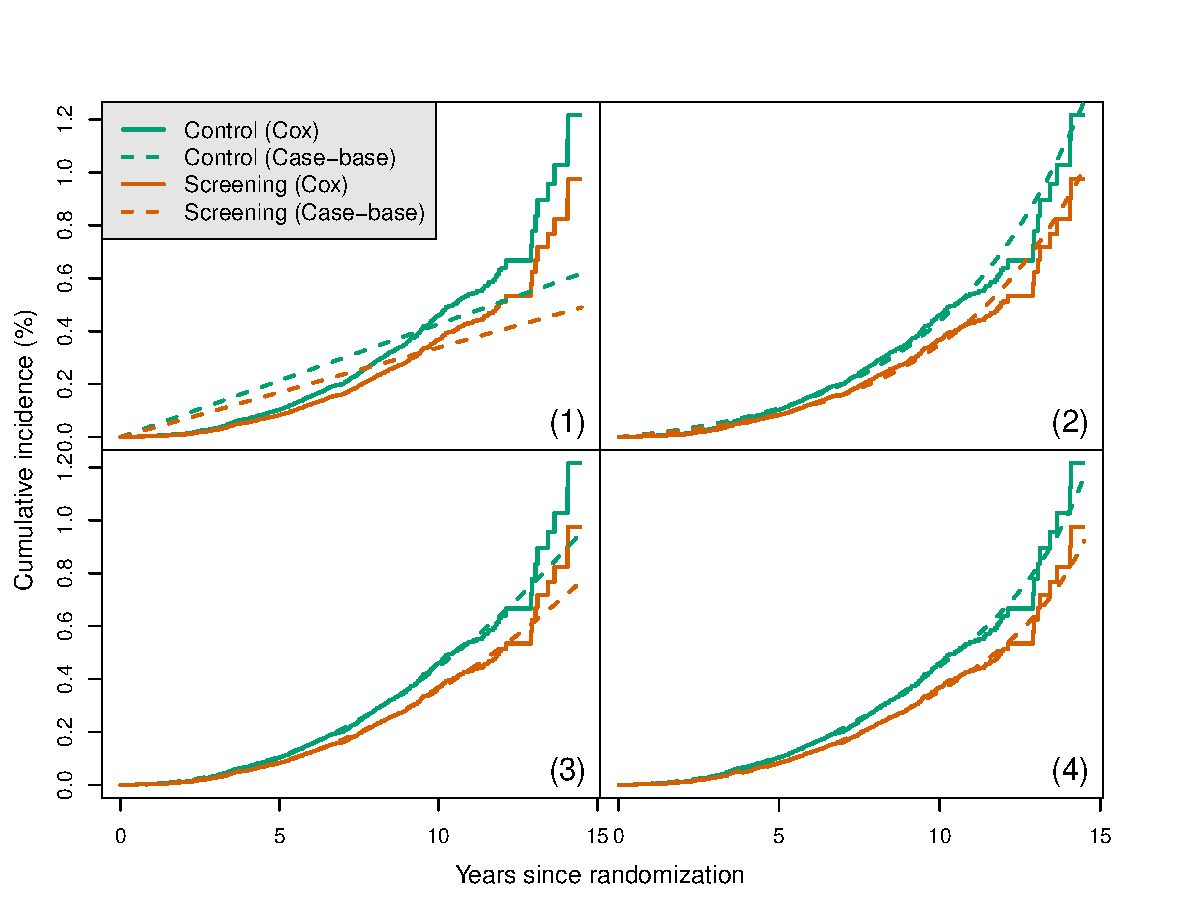
\includegraphics[width=\textwidth,keepaspectratio=true]{../figures/erspc-cox-cif-1} 

}

\caption{CIFs for control and screening groups in the ERSPC data. In each of the panels, we plot the CIF from the Cox model using \code{survival::survfit} (solid line) and the CIF from the case-base sampling scheme (dashed line) with different functional forms of time. (1) The time variable is excluded (exponential). (2) Linear function of time (Gompertz). (3) The natural logarithm (Weibull). (4) Cubic B-spline expansion of time.}\label{fig:erspc-cox-cif}
\end{figure}
\end{CodeChunk}

In the following table, we present a side-by-side comparison of the
hazard ratios and confidence intervals estimated from
\code{fitSmoothHazard} and the corresponding parametric model using
\code{survival::survreg}, as well as the Cox model estimate. The hazard
ratio estimates and confidence intervals are similar across all four
models. This reinforces the idea that, under proportional hazards, we do
not need to model the full hazard to obtain reliable estimates of the
hazard ratio. Nevertheless, Figure \ref{fig:erspc-cox-cif} shows that
different parametric models can still give rise to qualitatively
different estimates for the CIF.

\begin{CodeChunk}
\begin{table}

\caption{\label{tab:print-erspc-estimates}Comparison of estimated hazard ratios and 95\% confidence intervals for ERSPC data.}
\centering
\begin{tabular}[t]{>{\bfseries}lcc}
\toprule
Model & casebase::fitSmoothHazard & survival::survreg\\
\midrule
Exponential & 0.81 (0.68, 0.96) & 0.81 (0.68, 0.96)\\
\cmidrule{1-3}
Gompertz & 0.79 (0.66, 0.94) & 0.80 (0.67, 0.95)\\
\cmidrule{1-3}
Weibull & 0.81 (0.68, 0.96) & 0.80 (0.65, 0.96)\\
\cmidrule{1-3}
Splines & 0.81 (0.68, 0.96) & --\\
\bottomrule
\multicolumn{3}{l}{Cox model estimate: HR (95\% CI) = 0.80 (0.67, 0.95)}\\
\end{tabular}
\end{table}

\end{CodeChunk}

With this first case study, we explored how \pkg{casebase} allows us to
fit different parametric survival models, and how we can compare the fit
of each model with tools from GLMs.

\hypertarget{case-study-2bone-marrow-transplant}{%
\section{Case study 2---Bone-marrow
transplant}\label{case-study-2bone-marrow-transplant}}

In the next case study, we show how case-base sampling can be used in
the context of a competing risk analysis. For illustrative purposes, we
will use the same data that was used in Scrucca \emph{et al}
\citeyearpar{scrucca2010regression}. The data was downloaded from the
first author's website, and it is now available as part of the
\pkg{casebase} package.

The data contains information on 177 patients who received a stem-cell
transplant for acute leukemia. The event of interest is relapse, but
other competing causes (e.g.~transplant-related death) were also
recorded. Several covariates were captured at baseline: sex, disease
type (acute lymphoblastic or myeloblastic leukemia, abbreviated as ALL
and AML, respectively), disease phase at transplant (Relapse, CR1, CR2,
CR3), source of stem cells (bone marrow and peripheral blood, coded as
BM+PB, or only peripheral blood, coded as PB), and age.

First, we can look at a population-time plot to visualize the incidence
density of both relapse and the competing events. In Figure
\ref{fig:compPop}, failure times are highlighted on the plot using red
dots for the event of interest (panel A) and blue dots for competing
events (panel B). In both panels, we see evidence of a non-constant
hazard function: the density of points is larger at the beginning of
follow-up than at the end.

\begin{CodeChunk}
\begin{figure}

{\centering 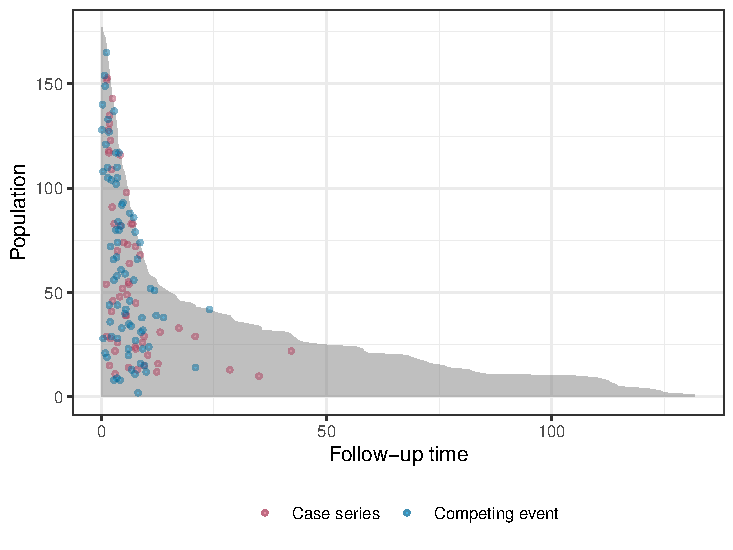
\includegraphics[width=\textwidth,keepaspectratio=true]{../figures/compPop-1} 

}

\caption[Population-time plot for the stem-cell transplant study with both relapse and competing events]{Population-time plot for the stem-cell transplant study with both relapse and competing events.}\label{fig:compPop}
\end{figure}
\end{CodeChunk}

Our main objective is to compute the absolute risk of relapse for a
given set of covariates. We start by fitting a smooth hazard to the data
using a linear term for time:

We will compare our hazard ratio estimates to that obtained from a Cox
regression. To do so, we need to treat the competing event as censoring.

\begin{CodeChunk}

\begin{CodeInput}
R> library(survival)
R> # Treat competing event as censoring
R> model_cox <- coxph(Surv(ftime, Status == 1) ~ Sex + D + Phase + Source + Age,
R+   data = bmtcrr
R+ )
\end{CodeInput}
\end{CodeChunk}

\begin{CodeChunk}
\begin{table}

\caption{\label{tab:bmtcrr-cis}Estimates and confidence intervals for the hazard ratios for each coefficient. Both estimates from case-base sampling and Cox regression are presented.}
\centering
\begin{tabular}[t]{lrlrl}
\toprule
\multicolumn{1}{c}{ } & \multicolumn{2}{c}{Case-Base} & \multicolumn{2}{c}{Cox} \\
\cmidrule(l{3pt}r{3pt}){2-3} \cmidrule(l{3pt}r{3pt}){4-5}
Covariates & HR & 95\% CI & HR & 95\% CI\\
\midrule
Sex & 0.70 & (0.4, 1.23) & 0.68 & (0.39, 1.19)\\
Disease & 0.53 & (0.29, 0.95) & 0.52 & (0.29, 0.93)\\
Phase (CR2 vs. CR1) & 1.12 & (0.45, 2.78) & 1.21 & (0.48, 3.02)\\
Phase (CR3 vs. CR1) & 1.45 & (0.37, 5.66) & 1.67 & (0.43, 6.5)\\
Phase (Relapse vs. CR1) & 4.04 & (1.88, 8.68) & 4.55 & (2.09, 9.9)\\
\addlinespace
Source & 1.48 & (0.48, 4.54) & 1.46 & (0.47, 4.54)\\
Age & 0.99 & (0.97, 1.01) & 0.99 & (0.97, 1.02)\\
\bottomrule
\end{tabular}
\end{table}

\end{CodeChunk}

From the fit object, we can extract both the hazard ratios and their
corresponding confidence intervals. These quantities appear in Table
\ref{tab:bmtcrr-cis}. As we can see, the only significant hazard ratio
identified by case-base sampling is the one associated with the phase of
the disease at transplant. More precisely, being in relapse at
transplant is associated with a hazard ratio of 3.89 when compared to
CR1.

Given the estimate of the hazard function obtained using case-base
sampling, we can compute the absolute risk curve for a fixed covariate
profile. We perform this computation for a 35 year old woman who
received a stem-cell transplant from peripheral blood at relapse. We
compared the absolute risk curve for such a woman with ALL with that for
a similar woman with AML. We will estimate the curve from 0 to 60
months.

We will compare our estimates to that obtained from a corresponding
Fine-Gray model \citeyearpar{fine1999proportional}. The Fine-Gray model
is a semiparametric model for the cause-specific \emph{subdistribution},
i.e.~the function \(f_k(t)\) such that
\[CI_k(t) =1 - \exp\left( - \int_0^t f_k(u) \textrm{d}u \right),\] where
\(CI_k(t)\) is the cause-specific cumulative incidence. The Fine-Gray
model allows to directly assess the effect of a covariate on the
subdistribution, as opposed to the hazard. For the computation, we will
use the \pkg{timereg} package \citep{timereg}:

\begin{CodeChunk}

\begin{CodeInput}
R> library(timereg)
R> model_fg <- comp.risk(Event(ftime, Status) ~ const(Sex) + const(D) +
R+                         const(Phase) + const(Source) + const(Age),
R+                       data = bmtcrr, cause = 1, model = "fg")
R> 
R> # Estimate absolute risk curve
R> risk_fg <- predict(model_fg, newdata, times = time_points)
\end{CodeInput}
\end{CodeChunk}

\begin{CodeChunk}
\begin{figure}

{\centering 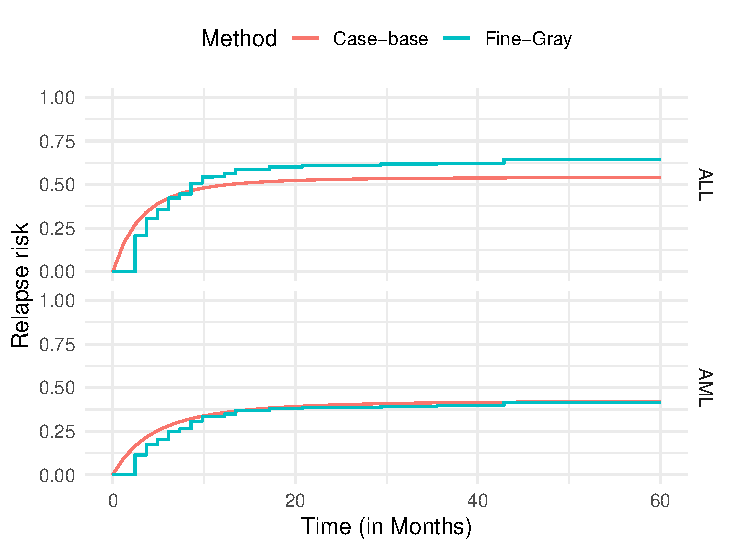
\includegraphics[width=\textwidth,keepaspectratio=true]{../figures/bmtcrr-risk-1} 

}

\caption{\label{fig:compAbsrisk} Absolute risk curve for a fixed covariate profile and the two disease groups. The estimate obtained from case-base sampling is compared to the Kaplan-Meier estimate.}\label{fig:bmtcrr-risk}
\end{figure}
\end{CodeChunk}

Figure \ref{fig:compAbsrisk} shows the absolute risk curves for both
case-base sampling and the Fine-Gray model. As we can see, the two
approaches agree quite well for AML; however, there seems to be a
difference of about 5\% between the two curves for ALL. This difference
does not appear to be significant: the curve from case-base sampling is
contained within a 95\% confidence band around the Fine-Gray absolute
risk curve (figure not shown).

\hypertarget{case-study-3support-data}{%
\section{Case study 3---SUPPORT Data}\label{case-study-3support-data}}

In the first two case studies, we described the basic functionalities of
the \pkg{casebase} package: creating population-time plots, fitting
parametric models for hazard functions, and estimating the corresponding
cumulative incidence curves. For the third case study, we show how
\pkg{casebase} can also be used for variable selection through
regularized estimation of the hazard function. To do this, we simply
replace logistic regression with a penalized counterpart. In
\pkg{casebase}, we achieve this by using the \pkg{glmnet} package
\citep{friedman2010jss}.

To illustrate this functionality, we use the dataset from the Study to
Understand Prognoses Preferences Outcomes and Risks of Treatment
(SUPPORT) \citep{knaus1995support}. The SUPPORT dataset tracks death in
five American hospitals within individuals who are considered seriously
ill.~The original data is available online from the Department of
Biostatistics at Vanderbilt University \citep{harrell_2020}. The cleaned
and imputed data consists of 9104 observations and 30 variables, and it
is available as part of the \pkg{casebase} package. For more information
about this dataset, the reader is encouraged to look at the
documentation in our package. A description of the variables can be
found in Table \ref{tab:support1}, and a breakdown of each categorical
variable appears in Table \ref{tab:support2}.

\begin{table}[ht]
\centering
\begin{tabular}{ccccc}
\hline
\textbf{Name} & \textbf{Labels}                          & \textbf{Levels} & \textbf{Storage} & \textbf{NAs} \\
\hline
age           & Age                                      &                 & double           & 0            \\
death         & Death at any time up to NDI date:31DEC94 &                 & double           & 0            \\
sex           &                                          & 2               & integer          & 0            \\
slos          & Days from Study Entry to Discharge       &                 & double           & 0            \\
d.time        & Days of Follow-Up                        &                 & double           & 0            \\
dzgroup       &                                          & 8               & integer          & 0            \\
dzclass       &                                          & 4               & integer          & 0            \\
num.co        & number of comorbidities                  &                 & double           & 0            \\
edu           & Years of Education                       &                 & double           & 202          \\
income        &                                          & 4               & integer          & 349          \\
scoma         & SUPPORT Coma Score based on Glasgow D3   &                 & double           & 0            \\
avtisst       & Average TISS, Days 3-25                  &                 & double           & 6            \\
race          &                                          & 5               & integer          & 5            \\
sps             & support physiology score day 3           &                   & double           & 1            \\
aps           & APS III no coma, imp bun,uout for ph1,D3 &                 & double           & 1            \\
hday            & Day in Hospital at Study Admit             &                 & double           & 0            \\ 
diabetes      & Diabetes (Com 27-28, Dx 73)              &                 & double           & 0            \\
dementia      & Dementia (Comorbidity 6)                 &                 & double           & 0            \\
ca              & Cancer State                             & 3               & integer          & 0            \\
meanbp        & Mean Arterial Blood Pressure Day 3       &                 & double           & 0            \\
wblc          & White Blood Cell Count Day 3             &                 & double           & 24           \\
hrt           & Heart Rate Day 3                         &                 & double           & 0            \\
resp          & Respiration Rate Day 3                   &                 & double           & 0            \\
temp          & Temperature (Celsius) Day 3              &                 & double           & 0            \\
pafi          & PaO2/(.01*FiO2) Day 3                    &                 & double           & 253          \\
alb           & Serum Albumin Day 3                      &                 & double           & 378          \\
bili          & Bilirubin Day 3                          &                 & double           & 297          \\
crea          & Serum creatinine Day 3                   &                 & double           & 3            \\
sod           & Serum sodium Day 3                       &                 & double           & 0            \\
ph            & Serum pH (arterial) Day 3                &                 & double           & 250          \\
glucose       & Glucose Day 3                            &                 & double           & 470          \\
bun           & BUN Day 3                                &                 & double           & 455          \\
urine         & Urine Output Day 3                       &                 & double           & 517          \\
adlp          & Activiites of Daily Living (ADL) Patient Day 3 &           & double           & 634          \\
adlsc         & Imputed ADL Calibrated to Surrogate      &                 & double           & 0           
\end{tabular}
\caption{Description of each variable in the SUPPORT dataset.}
\label{tab:support1}
\end{table}

\begin{table}[ht]
\centering
\begin{tabular}{cc}
\hline
\textbf{Variable} & \textbf{Levels}                      \\
\hline
sex      & female                                        \\
         & male                                          \\
dzgroup  & ARF/MOSF w/Sepsis                             \\
         & COPD                                          \\
         & CHF                                           \\
         & Cirrhosis                                     \\
         & Coma                                          \\
         & Colon Cancer                                  \\
         & Lung Cancer                                   \\
         & MOSF w/Malig                                  \\
dzclass  & ARF/MOSF                                      \\
         & COPD/CHF/Cirrhosis                            \\
         & Coma                                          \\
         & Cancer                                        \\
         & \textgreater{}\$50k                           \\
race     & white                                         \\
         & black                                         \\
         & asian                                         \\
         & other                                         \\
         & hispanic                                      \\
ca       & Yes                                           \\
         & No                                            \\
         & Metastatic                                    \\
\end{tabular}
\caption{Description of each level within each categorical variable in the SUPPORT dataset.}
\label{tab:support2}
\end{table}

In the original study, the authors developed two scores for predicting
the outcome. These scores are available as part of the data: SUPPORT day
3 physiology score (\code{sps}) and APACHE III day 3 physiology score
(\code{aps}). Using these scores, we will explore three Cox regression
scenarios as a baseline comparison for \pkg{casebase}: \code{sps} only,
\code{aps} only, and all covariates excluding \code{sps} and \code{aps}.
We will compare the three models using a time-dependent version of the
classical Brier score that is adjusted for censoring
\citep{graf1999ass}. The Brier score can be used to assess both
discrimination and calibration in a single model. Moreover, it provides
a metric that can be used to compare parametric and semi-parametric
survival models. To account for overfitting, we will use 95\% of the
observations to train our models, while the remaining 5\% will be used
to compute absolute risk curves and the Brier scores.

In Figure\ref{fig:brier1} (A), we can see that all Cox models have
similar average survival curves. On the other hand, Figure
\ref{fig:brier1} (B) shows that the full model has the lowest Brier
score overall. For this reason, we will use this model in our comparison
between regularized Cox regression, Kaplan-Meier estimation, and the
approach from \pkg{casebase}.

\begin{CodeChunk}
\begin{figure}

{\centering 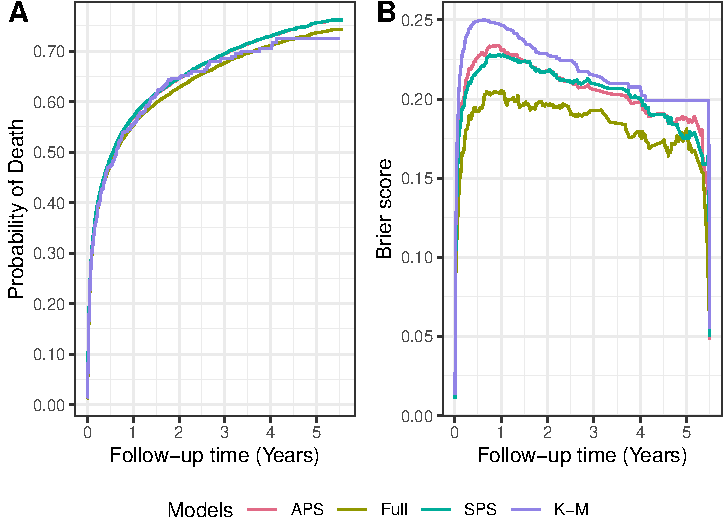
\includegraphics[width=\textwidth,keepaspectratio=true]{../figures/brierpt1-1} 

}

\caption{\label{fig:brier1} Comparison of three Cox regression models to the unadjusted Kaplan-Meier curve. (A) Cumulative Incidence curves. For a given model, the plotted curve is the average curve of each individual in the study. Each follow-up time seen in the study was used. There are minimal differences between the curves. APS coincides with the SPS curve, as they are considerably overlapped.(B) Time-dependent Brier scores, where a lower score is better. The full model performs best overall.}\label{fig:brierpt1}
\end{figure}
\end{CodeChunk}

For our penalized logistic regression model, we opt for the natural log
of time; recall that this corresponds to a Weibull distribution. For
fitting the penalized hazard, we use \code{fitSmoothHazard.fit}, which
is a matrix interface to the function \code{fitSmoothHazard}. In order
to use this interface, we first create a matrix \code{y} containing the
time and event variables, and a matrix \code{x} containing all remaining
covariates we would like to include in the model space. We used lasso
penalization by setting \code{alpha = 1}. Moreover, we use the argument
\code{penalty.factor} to force the time variable into the final model.

\begin{CodeChunk}

\begin{CodeInput}
R> x <- model.matrix(death ~ . - d.time - aps - sps, 
R+                   data = train)[, -c(1)] # Remove intercept
R> y <- data.matrix(subset(train, select = c(d.time, death)))
R> 
R> # Regularized logistic regression to estimate hazard
R> cbFull <- casebase::fitSmoothHazard.fit(x, y,
R+   family = "glmnet",
R+   time = "d.time", event = "death",
R+   formula_time = ~ log(d.time), alpha = 1,
R+   ratio = 10, standardize = TRUE,
R+   penalty.factor = c(0, rep(1, ncol(x)))
R+ )
\end{CodeInput}
\end{CodeChunk}

Next, we can use the object \code{cbFull} to estimate the absolute risk
curve on the test data. We first create a matrix \code{newx} containing
the relevant variables. Next, using \code{times}, we specify the time
points at which the cumulative incidence will be computed. Finally,
using the parameter \code{s = "lambda.1se"}, we specify at which value
of the tuning parameter we want to retrieve the coefficient estimates.

\begin{CodeChunk}

\begin{CodeInput}
R> # Estimating the absolute risk curve using the newdata parameter
R> newx <- model.matrix(death ~ . - d.time - aps - sps, 
R+                   data = test)[, -c(1)]
R> times <- sort(unique(test$d.time))
R> 
R> abCbFull <- casebase::absoluteRisk(cbFull,
R+   time = times,
R+   newdata = newx,
R+   s = "lambda.1se",
R+   method = "numerical"
R+ )
\end{CodeInput}
\end{CodeChunk}

Our first comparison plot examines the covariates that were selected
between all three hazard functions. Note that Cox regression without
penalization selected more covariates than the other two, but only the
intersection of coefficients with values greater than 0 are displayed in
\ref{fig:cs3lolliPlot}. A visible tendency is for Cox regression to have
larger estimated coefficients. This is expected, as there are no
restrictions on the size of coefficients. The smallest coefficient
estimates are found in penalized logistic model, aside from cancer state
(cano).

\begin{CodeChunk}
\begin{figure}

{\centering 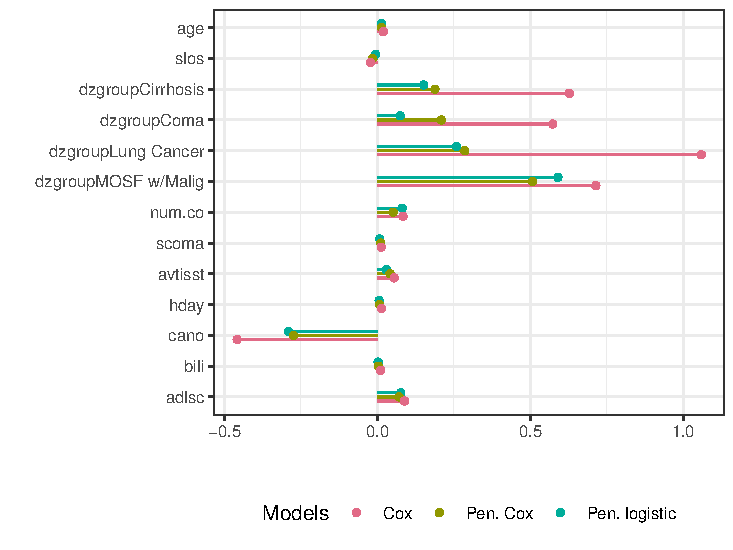
\includegraphics[width=\textwidth,keepaspectratio=true]{../figures/coefplots-1} 

}

\caption{\label{fig:cs3lolliPlot} Lollipop plot showing the coefficient estimates between three models. If a coefficient estimate is 0 in any model, it is removed from the plot for simplicity. Shrinkage occurs due to penalization.}\label{fig:coefplots}
\end{figure}
\end{CodeChunk}

These values do not inform us of model performance. To do so, we take
our hazard functions and use them to predict the absolute risk of
everyone in our test set, over time. The probabilities over time for
each individual are averaged, resulting in the absolute risk curves in
Figure \ref{fig:cs3FinalBrier} (A). There is separation between the
curves, but it is minimal. To better demonstrate the differences in
performance between the models, we compare Brier scores over time. In
Figure \ref{fig:cs3FinalBrier} (B), the Brier score is lower in our
penalized logistic regression model compared to both Cox regression
models. The differences, however, are minimal. All three outperform the
Kaplan-Meier model.

\begin{CodeChunk}
\begin{figure}

{\centering 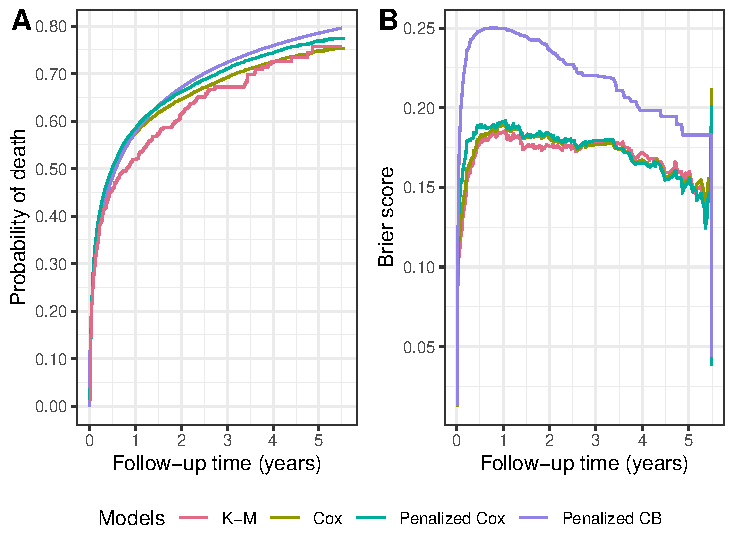
\includegraphics[width=\textwidth,keepaspectratio=true]{../figures/riskregressionBrier-1} 

}

\caption{\label{fig:cs3FinalBrier} (A) Four curves comparing the probabilities of death as it changes over follow-up time between Cox regression, penalized Cox regression, penalized logistic regression, and Kaplan-Meier. All follow-up times seen in the new data were used. (B) Four curves demonstrating the Brier scores as they change over time between Cox regression, penalized Cox regression, penalized logistic regression, and Kaplan-Meier. Lower is better. Penalized logistic regression produced the lowest results over follow-up time.}\label{fig:riskregressionBrier}
\end{figure}
\end{CodeChunk}

\hypertarget{case-study-4stanford-heart-transplant-data}{%
\section{Case study 4---Stanford Heart Transplant
Data}\label{case-study-4stanford-heart-transplant-data}}

In the previous case studies, we only considered covariates that were
fixed at baseline. In this next case study, we will use the Stanford
Heart Transplant data
\citep[\citet{crowley1977covariance}]{clark1971cardiac} to show how
case-base sampling can also be used in the context of time-varying
covariates. As an example that already appeared in the literature,
case-base sampling was used to study vaccination safety, where the
exposure period was defined as the week following vaccination
\citep{saarela2015case}. Hence, the main covariate of interest,
i.e.~exposure to the vaccine, was changing over time. In this context,
case-base sampling offers an efficient alternative to nested
case-control designs or self-matching.

Recall the setting of Stanford Heart Transplant study: patients were
admitted to the Stanford program after meeting with their physician and
determining that they were unlikely to respond to other forms of
treatment. After enrollment, the program searched for a suitable donor
for the patient, which could take anywhere between a few days to almost
a year. We are interested in the effect of a heart transplant on
survival; therefore, the patient is considered exposed only after the
transplant has occurred.

As before, we can look at the population-time plot for a graphical
summary of the event incidence. As we can see, most events occur early
during the follow-up period, and therefore we do not expect the hazard
to be constant.

\begin{CodeChunk}


\begin{center}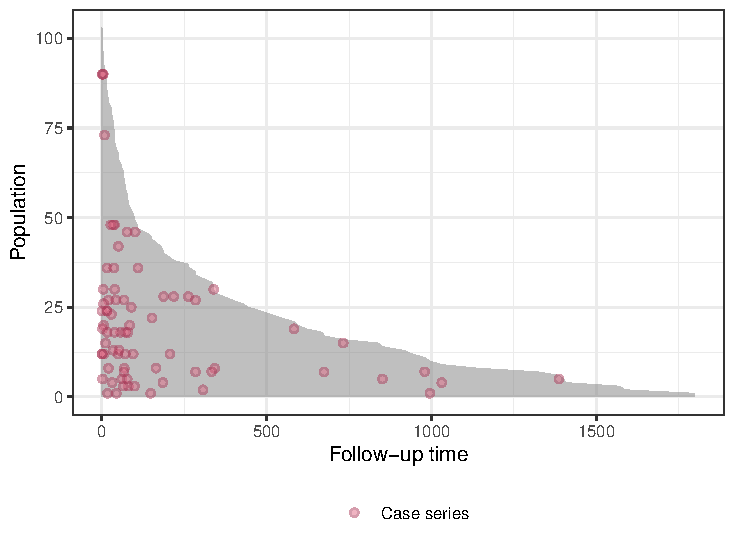
\includegraphics[width=\textwidth,keepaspectratio=true]{../figures/stanford-poptime-1} \end{center}

\end{CodeChunk}

Since the exposure is time-dependent, we need to manually define the
exposure variable \emph{after} case-base sampling and \emph{before}
fitting the hazard function. For this reason, we will use the
\texttt{sampleCaseBase} function directly.

Next, we will compute the number of days from acceptance into the
program to transplant, and we use this variable to determine whether
each population-moment is exposed or not.

Finally, we can fit the hazard using various linear predictors.

Note that the fourth model includes an interaction term between exposure
and follow-up time. In other words, this model no longer exhibit
proportional hazards. The evidence of non-proportionality of hazards in
the Stanford Heart Transplant data has been widely discussed
\citep{arjas1988graphical}.

We can then compare the goodness of fit of these four models using the
Akaike Information Criterion (AIC).

\begin{CodeChunk}

\begin{CodeOutput}
#> Model1 Model2 Model3 Model4 
#>    491    459    444    445
\end{CodeOutput}
\end{CodeChunk}

As we can, the best fit is the fourth model. By visualizing the hazard
functions for both exposed and unexposed individuals, we can more
clearly see how the hazards are no longer proportional.

\begin{CodeChunk}

\begin{CodeInput}
R> # Compute hazards---
R> # First, create a list of time points for both exposure status
R> hazard_data <- expand.grid(
R+   exposure = c(0, 1),
R+   futime = seq(0, 425,
R+     length.out = 100
R+   )
R+ )
R> 
R> # Set the offset to zero
R> hazard_data$offset <- 0
R> # Use predict to get the fitted values, and exponentiate to
R> # transform to the right scale
R> hazard_data$hazard <- exp(predict(fit4,
R+   newdata = hazard_data,
R+   type = "link"
R+ ))
R> # Add labels for plots
R> hazard_data$Status <- factor(hazard_data$exposure,
R+   labels = c("NoTrans", "Trans")
R+ )
R> 
R> ggplot(hazard_data, aes(futime, hazard, colour = Status)) +
R+   geom_line() +
R+   paper_gg_theme +  
R+   ylab("Hazard") +
R+   xlab("Follow-up time")
\end{CodeInput}


\begin{center}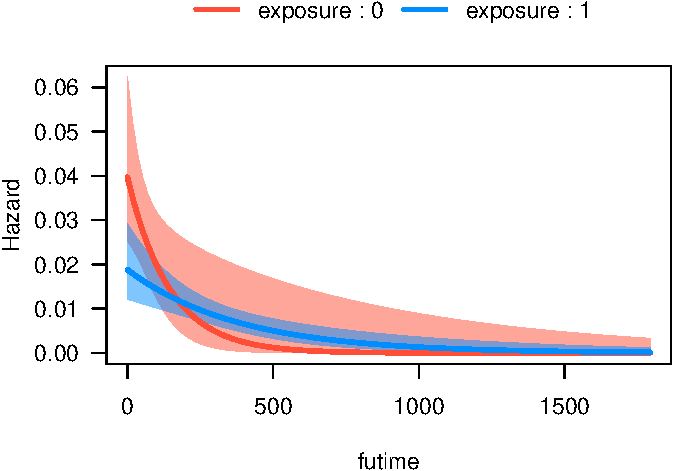
\includegraphics[width=\textwidth,keepaspectratio=true]{../figures/stanford-hazard-1} \end{center}

\end{CodeChunk}

The non-proportionality seems to be more pronounced at the beginning of
follow-up than the end. Finally, we can turn these estimates of the
hazard function into estimates of the cumulative incidence functions.

\begin{CodeChunk}

\begin{CodeOutput}
#> [1] "absRiskCB" "matrix"    "array"
\end{CodeOutput}


\begin{center}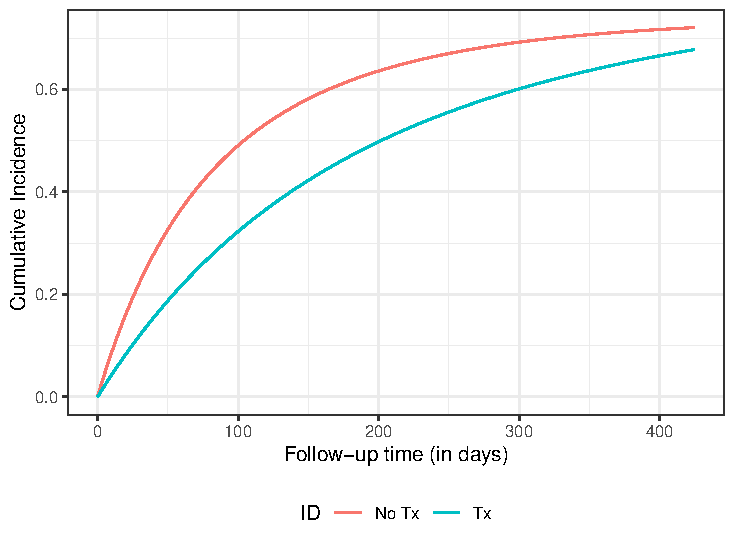
\includegraphics[width=\textwidth,keepaspectratio=true]{../figures/stanford-risk-1} \end{center}

\end{CodeChunk}

Note that we can easily adapt the code above to the situation where a
patient receives a heart transplant at a point in time of interest, for
example after 30 days.

\begin{CodeChunk}


\begin{center}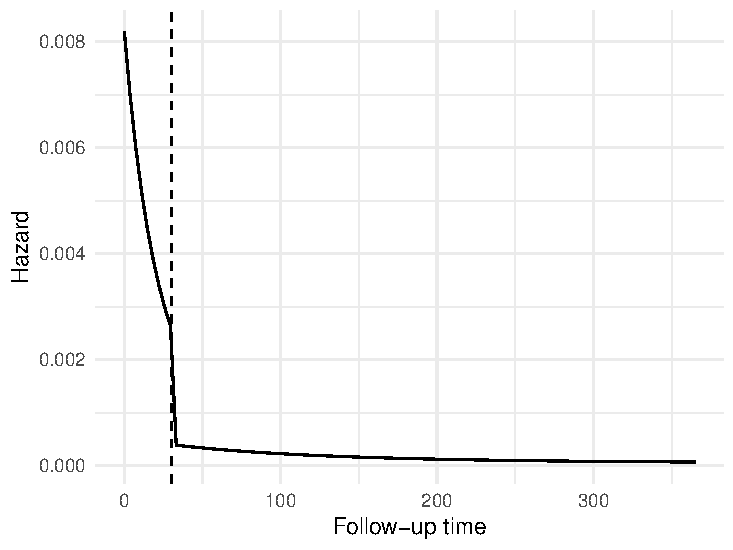
\includegraphics[width=\textwidth,keepaspectratio=true]{../figures/stanford-1y-haz-1} \end{center}

\end{CodeChunk}

We can then compare the 1-year mortality risk without transplant and
with transplant at 30 days.

\begin{CodeChunk}

\begin{CodeOutput}
#>  time     
#>     0 0.00
#>   365 0.72
\end{CodeOutput}

\begin{CodeOutput}
#> [1] 0.65
\end{CodeOutput}
\end{CodeChunk}

As we can see, the risk estimate at 1-year is about 30\% lower if the
patient receives a heart transplant at 30 days.

We can also plot the hazard ratio:

\begin{CodeChunk}


\begin{center}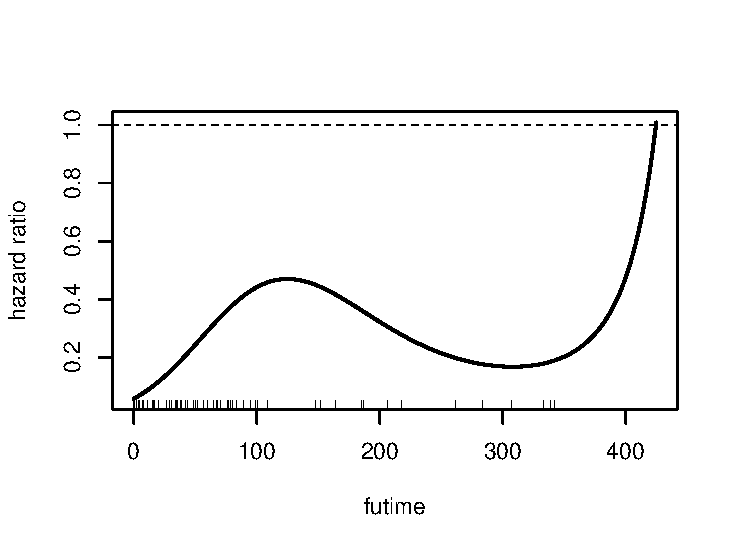
\includegraphics[width=\textwidth,keepaspectratio=true]{../figures/unnamed-chunk-12-1} \end{center}

\end{CodeChunk}

\hypertarget{discussion}{%
\section{Discussion}\label{discussion}}

In this article, we presented the \proglang{R} package \pkg{casebase},
which provides functions for fitting smooth parametric hazards and
estimating CIFs using case-base sampling. Our package also provide
several functions to produce graphical summaries of the data and the
results. We outlined the theoretical underpinnings of the approach, we
provided details about our implementation, and we illustrated the merits
of the approach and the package through four case studies.

As a methodological framework, case-base sampling is very flexible. This
flexibility has been explored before in the literature: for example,
Saarela and Hanley \citeyearpar{saarela2015case} used case-base sampling
to model a time-dependent exposure variable in a vaccine safety study.
As another example, Saarela and Arjas \citeyearpar{saarela2015non}
combined case-base sampling and a Bayesian non-parametric framework to
compute individualized risk assessments for chronic diseases. In the
case studies above, we further explored this flexibility along two
fronts. On the one hand, we showed how splines could be used as part of
the linear predictor to model the effect of time on the hazard. This
strategy yielded estimates of the survival function that were
qualitatively similar to semiparametric estimates derived from Cox
regression; however, case-base sampling led to estimates of the survival
function that \emph{vary smoothly in time} and are thus easier to
interpret. On the other hand, we also displayed the flexibility of
case-base sampling by showing how it could be combined with penalized
logistic regression to perform variable selection. Even though we did
not illustrate it in this article, case-base sampling can also be
combined with the framework of \emph{generalized additive models}. This
functionality has already been implemented in the package. Similarly,
case-base sampling can be combined with quasi-likelihood estimation to
fit survival models that can account for the presence of
over-dispersion. All of these examples illustrate how the case-base
sampling framework in general, and the package \pkg{casebase} in
particular, allows the user to fit a broad and flexible family of
survival functions.

As presented in Hanley \& Miettinen \citeyearpar{hanley2009fitting},
case-base sampling is comprised of three steps: 1) sampling a case
series and a base series from the study; 2) fit the log-hazard as a
linear function of predictors (including time); and 3) use the fitted
hazard to estimate the CIF. Accordingly, our package provides functions
for each step. Moreover, the simple interface of the
\code{fittingSmoothHazard} function resembles the \code{glm} interface.
This interface should look familiar to new users. Our modular approach
also provides a convenient way to extend our package for new sampling or
fitting strategies.

In the case studies above, we compared the performance of case-base
sampling with that of Cox regression and Fine-Gray models. In terms of
function interface, \pkg{casebase} uses a formula interface that is
closer to that of \code{glm}, in that the event variable is the only
variable appearing on the left-hand side of the formula. By contrast,
both \code{survival::coxph} and \code{timereg::comp.risk} use arrays
that capture both the event type and time. Both approaches to modeling
yield user-friendly code. However, in terms of output, both approaches
differ significantly. Case-base sampling produces smooth hazards and
smooth cumulative incidence curves, whereas Cox regression and Fine-Gray
models produce step-wise CIFs and never explicitly model the hazard
function. Qualitatively, we showed that by using splines in the linear
predictor, all three models yielded similar curves. However, the smooth
nature of the output of \pkg{casebase} provides a more intuitive
interpretation for consumers of these predictions. In Table
\ref{tab:compCBvsCox}, we provide a side-by-side comparison between the
Cox model and case-base sampling.

\begin{table}
\caption{\label{tab:compCBvsCox}Comparison between the Cox model and case-base sampling}
\centering
\begin{tabular}[t]{llp{5cm}}
\toprule
Feature & Cox model & Case-base sampling\\
\midrule
Model type & Semi-parametric & Fully parametric\\
Time & Left hand side of the formula & Right hand side (allows flexible modeling of time)\\
Cumulative incidence & Step function & Smooth-in-time curve\\
Non-proportional hazards & Interaction of covariates with time & Interaction of covariates with time\\
Model testing &  & Use GLM framework \newline (e.g.\ LRT, AIC, BIC)\\
\addlinespace
Competing risks & Difficult & Cause-specific CIFs\\
% Prediction & Kaplan-Meier-based & ROC, AUC, risk reclassification probabilities\\
\bottomrule
\end{tabular}
\end{table}

Our choice of modeling the log-hazard as a linear function of covariates
allows us to develop a simple computational scheme for estimation.
However, as a downside, it does not allow us to model location and scale
parameters separately like the package \pkg{flexsurv}. For example, if
we look at the Weibull distribution as parametrised in
\code{stats::pweibull}, the log-hazard function is given by
\[ \log \lambda(t; \alpha, \beta) = \left[\log(\alpha/\beta) - (\alpha - 1)\log(\beta)\right] + (\alpha - 1)\log t,\]
where \(\alpha,\beta\) are shape and scale parameters, respectively.
Unlike \pkg{casebase}, the approach taken by \pkg{flexsurv} also allows
the user to model the scale parameter as a function of covariates. Of
course, this added flexibility comes at the cost of interpretability: by
modeling the log-hazard directly, the parameter estimates from
\pkg{casebase} can be interpreted as estimates of log-hazard ratios. To
improve the flexibility of \pkg{casebase} at capturing the scale of a
parametric family, we could replace the logistic regression with its
quasi-likelihood counterpart and therefore model over- and
under-dispersion with respect to the logistic likelihood. We defer the
study of the properties and performance of such a model to a future
article.

Future work will look at some of the methodological extensions of
case-base sampling. First, to assess the quality of the model fit, we
would like to study the properties of the residuals (e.g.~Cox-Snell,
martingale). More work needs to be done to understand these residuals in
the context of the partial likelihood underlying case-base sampling. The
resulting diagnostic tools could then be integrated in this package.
Also, we are interested in extending case-base sampling to account for
interval censoring. This type of censoring is very common in
longitudinal studies, and many packages (e.g.~\pkg{SmoothHazard},
\pkg{survival} and \pkg{rstpm2}) provide functions to account for it.
Again, we hope to include any resulting methodology as part of this
package.

In future versions of the package, we also want to increase the
complement of diagnostic and inferential tools that are currently
available. For example, we would like to include the ability to compute
confidence intervals for the cumulative incidence curve. The delta
method or parametric bootstrap are two different strategies we can use
to construct approximate confidence intervals. Furthermore, we would
like to include more functions to compute calibration and discrimination
statistics (e.g.~AUC) for our models. Saarela and Arjas
\citeyearpar{saarela2015non} also describe how to obtain a posterior
distribution for the AUC from their model. Their approach could
potentially be included in \pkg{casebase}. Finally, we want to provide
more flexibility in how the case-base sampling is performed. This could
be achieved by adding a \code{hazard} argument to the function
\code{sampleCaseBase}. In this way, users could specify their own
sampling mechanism. For example, they could provide a hazard that gives
sampling probabilities that are proportional to the cardiovascular
disease event rate given by the Framingham score \citep{saarela2015non}.

In conclusion, we presented the \proglang{R} package \pkg{casebase}
which implements case-base sampling for fitting parametric survival
models and for estimating smooth cumulative incidence functions using
the framework of generalized linear models. We strongly believe that its
flexibility and its foundation on the familiar logistic regression model
will make it appealing to new and established practitioners.

\hypertarget{environment-details}{%
\section{Environment Details}\label{environment-details}}

This report was generated on 2020-08-04 09:28:27 using the following
computational environment and dependencies:

\begin{CodeChunk}

\begin{CodeOutput}
#> R version 4.0.2 (2020-06-22)
#> Platform: x86_64-pc-linux-gnu (64-bit)
#> Running under: Pop!_OS 20.04 LTS
#> 
#> Matrix products: default
#> BLAS:   /usr/lib/x86_64-linux-gnu/blas/libblas.so.3.9.0
#> LAPACK: /usr/lib/x86_64-linux-gnu/lapack/liblapack.so.3.9.0
#> 
#> locale:
#>  [1] LC_CTYPE=en_US.UTF-8       LC_NUMERIC=C              
#>  [3] LC_TIME=en_US.UTF-8        LC_COLLATE=en_US.UTF-8    
#>  [5] LC_MONETARY=en_US.UTF-8    LC_MESSAGES=en_US.UTF-8   
#>  [7] LC_PAPER=en_US.UTF-8       LC_NAME=C                 
#>  [9] LC_ADDRESS=C               LC_TELEPHONE=C            
#> [11] LC_MEASUREMENT=en_US.UTF-8 LC_IDENTIFICATION=C       
#> 
#> attached base packages:
#> [1] splines   stats     graphics  grDevices utils     datasets  methods  
#> [8] base     
#> 
#> other attached packages:
#>  [1] broom_0.7.0               dotwhisker_0.5.0         
#>  [3] timereg_1.9.6             glue_1.4.1               
#>  [5] scales_1.1.1              forcats_0.5.0            
#>  [7] stringr_1.4.0             dplyr_1.0.0              
#>  [9] purrr_0.3.4               readr_1.3.1              
#> [11] tidyr_1.1.0               ggplot2_3.3.2            
#> [13] tidyverse_1.3.0           lubridate_1.7.9          
#> [15] visreg_2.7.0              tibble_3.0.3             
#> [17] riskRegression_2020.06.25 prodlim_2019.11.13       
#> [19] flexsurv_1.1.1            survival_3.2-3           
#> [21] pracma_2.2.9              magrittr_1.5             
#> [23] kableExtra_1.1.0          glmnet_4.0-2             
#> [25] Matrix_1.2-18             data.table_1.13.0        
#> [27] cowplot_1.0.0             colorspace_1.4-1         
#> [29] casebase_0.9.0           
#> 
#> loaded via a namespace (and not attached):
#>  [1] TH.data_1.0-10      VGAM_1.1-3          ellipsis_0.3.1     
#>  [4] ggstance_0.3.4      htmlTable_2.0.1     fs_1.4.2           
#>  [7] base64enc_0.1-3     rstudioapi_0.11     farver_2.0.3       
#> [10] MatrixModels_0.4-1  fansi_0.4.1         mvtnorm_1.1-1      
#> [13] xml2_1.3.2          codetools_0.2-16    knitr_1.29         
#> [16] Formula_1.2-3       jsonlite_1.7.0      cluster_2.1.0      
#> [19] dbplyr_1.4.4        png_0.1-7           compiler_4.0.2     
#> [22] httr_1.4.2          backports_1.1.8     assertthat_0.2.1   
#> [25] cli_2.0.2           acepack_1.4.1       htmltools_0.5.0    
#> [28] quantreg_5.61       tools_4.0.2         gtable_0.3.0       
#> [31] Rcpp_1.0.5          cellranger_1.1.0    vctrs_0.3.2        
#> [34] nlme_3.1-148        conquer_1.0.1       iterators_1.0.12   
#> [37] xfun_0.16           rvest_0.3.5         lifecycle_0.2.0    
#> [40] polspline_1.1.19    muhaz_1.2.6.1       MASS_7.3-51.6      
#> [43] zoo_1.8-8           hms_0.5.3           sandwich_2.5-1     
#> [46] SparseM_1.78        RColorBrewer_1.1-2  rticles_0.14       
#> [49] yaml_2.2.1          gridExtra_2.3       rms_6.0-1          
#> [52] rpart_4.1-15        latticeExtra_0.6-29 stringi_1.4.6      
#> [55] foreach_1.5.0       checkmate_2.0.0     lava_1.6.7         
#> [58] shape_1.4.4         mets_1.2.7.1        rlang_0.4.7        
#> [61] pkgconfig_2.0.3     matrixStats_0.56.0  evaluate_0.14      
#> [64] lattice_0.20-41     labeling_0.3        htmlwidgets_1.5.1  
#> [67] cmprsk_2.2-10       tidyselect_1.1.0    deSolve_1.28       
#> [70] R6_2.4.1            generics_0.0.2      Hmisc_4.4-0        
#> [73] multcomp_1.4-13     DBI_1.1.0           withr_2.2.0        
#> [76] pillar_1.4.6        haven_2.3.1         foreign_0.8-80     
#> [79] mgcv_1.8-31         nnet_7.3-14         mstate_0.2.12      
#> [82] modelr_0.1.8        crayon_1.3.4        rmarkdown_2.3      
#> [85] jpeg_0.1-8.1        grid_4.0.2          readxl_1.3.1       
#> [88] blob_1.2.1          reprex_0.3.0        digest_0.6.25      
#> [91] webshot_0.5.2       numDeriv_2016.8-1.1 stats4_4.0.2       
#> [94] munsell_0.5.0       viridisLite_0.3.0   quadprog_1.5-8
\end{CodeOutput}
\end{CodeChunk}

The current Git commit details are:

\begin{CodeChunk}

\begin{CodeOutput}
#> Local:    master /home/jesseislam/Documents/gits/cbpaper
#> Remote:   master @ origin (git@github.com:Jesse-Islam/cbpaper.git)
#> Head:     [c4450d3] 2020-07-28: Vetted lit-rev, fig and fig comments (cs3)
\end{CodeOutput}
\end{CodeChunk}

\bibliography{references.bib}


\end{document}

